%-------------------------------------------------------------------------------
%	PACKAGES AND THEMES
%-------------------------------------------------------------------------------
\documentclass[xcolor=dvipsnames]{beamer}
\mode<presentation> {}
% The Beamer class comes with a number of default slide themes
% which change the colors and layouts of slides. Below this is a list
% of all the themes, uncomment each in turn to see what they look like.
%\usetheme{default}
%\usetheme{AnnArbor}
\usetheme{Antibes}
%\usetheme{Bergen}
%\usetheme{Berkeley}
%\usetheme{Berlin}
%\usetheme{Boadilla}
%\usetheme{CambridgeUS}
%\usetheme{Copenhagen}
%\usetheme{Darmstadt}
%\usetheme{Dresden}
%\usetheme{Frankfurt}
%\usetheme{Goettingen}
%\usetheme{Hannover}
%\usetheme{Ilmenau}
%\usetheme{JuanLesPins}
%\usetheme{Luebeck}
%\usetheme{Madrid}
%\usetheme{Malmoe}
%\usetheme{Marburg}
%\usetheme{Montpellier}
%\usetheme{PaloAlto}
%\usetheme{Pittsburgh}
%\usetheme{Rochester}
%\usetheme{Singapore}
%\usetheme{Szeged}
%\usetheme{Warsaw}
\usepackage{blkarray}
\usepackage{amsmath}
\usepackage{graphicx}
\usepackage{xfrac}
\usepackage{xcolor}
%\usepackage{kbordermatrix}

\definecolor{alt}{rgb}{0.44,0.00,0.16} % SET THIS TO A WARM RED WITH RGB VALUES
%\setbeamercolor{alerted text}{fg=alt,bg=}
\setbeamercolor{alerted text}{fg=purple,bg=}

\AtBeginSection{\frame{\tableofcontents[currentsection]}}

\graphicspath{ {img/} }		% Images live here

\title[Lord's Paradox]{Lord's Paradox}

\author{JCSzamosi}
\institute[FMF]{McMaster University Farncombe Metagenomics Facility}

\date{\today}
\begin{document}

%\begin{withoutheadline}
\begin{frame}
\titlepage
\end{frame}

\begin{frame}[plain]
\tableofcontents
\end{frame}
%\end{withoutheadline}

\section{Lord's Formulation}
\begin{frame}
``A large university is interested in investigating the effects on the students
of the diet provided in the university dining halls and any sex differences in
these effects. Various types of data are gathered. In particular, the weight of
each student at the time of his arrival in September and his weight the
following June are recorded.'' (Lord 1967, p. 304)
\end{frame}

\section{Mediation}
\begin{frame}
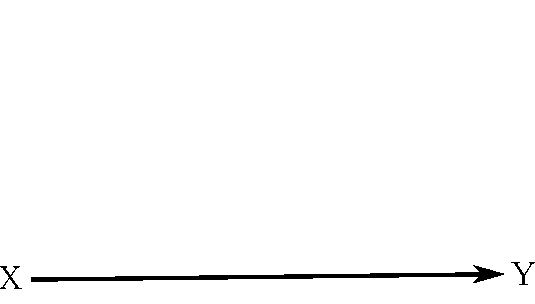
\includegraphics{arrow_diag_1.pdf}
\end{frame}

\begin{frame}{}
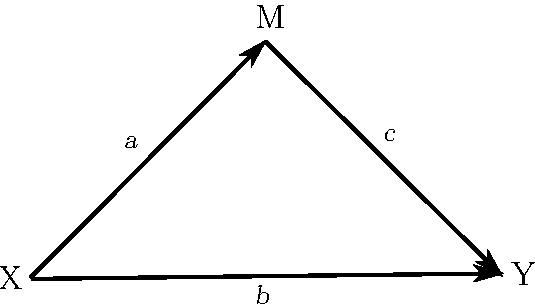
\includegraphics{arrow_diag_2.pdf}
\end{frame}

\begin{frame}{}
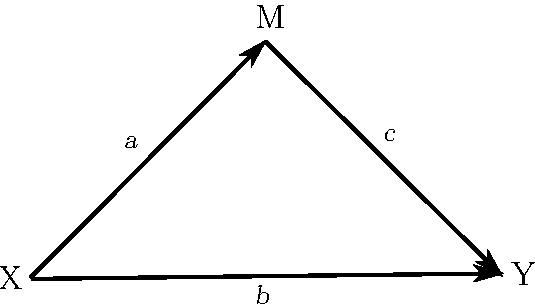
\includegraphics{arrow_diag_2.pdf}
\begin{itemize}
	\item \textbf{Total Effect} of X on Y includes the portion of the effect
	mediated by M
	\item \textbf{Direct Effect} is only the part that is \textit{not} mediated
	by M
\end{itemize} 
\end{frame}

\begin{frame}{}
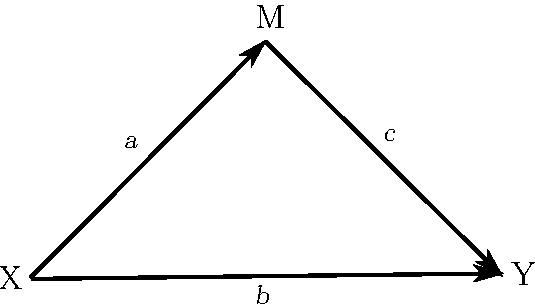
\includegraphics{arrow_diag_2.pdf}
\begin{itemize}
	\item \textbf{Total Effect} $TE = (b + ac) - a$ or, rearranged $TE = b - a(1
	- c)$
	\item \textbf{Direct Effect} $DE = b$
\end{itemize} 
\end{frame}

\end{document}
